\documentclass[nooutcomes]{ximera}
%\documentclass[space,handout,nooutcomes]{ximera}

% For preamble materials

\usepackage{pgf,tikz}
\usepackage{mathrsfs}
\usetikzlibrary{arrows}
\usepackage{framed}
\usepackage{amsmath}
\pgfplotsset{compat=1.17}

\def\fixnote#1{\begin{framed}{\textcolor{red}{Fix note: #1}}\end{framed}}  % Allows insertion of red notes about needed edits
%\def\fixnote#1{}

\def\detail#1{{\textcolor{blue}{Detail: #1}}}   

\pdfOnly{\renewenvironment{image}[1][]{\begin{center}}{\end{center}}}

\graphicspath{
  {./}
  {chapter1/}
  {chapter2/}
  {chapter4/}
  {proofs/}
  {graphics/}
  {../graphics/}
}

\newenvironment{sectionOutcomes}{}{}


%%% This set of code is all of our user defined commands
\newcommand{\bysame}{\mbox{\rule{3em}{.4pt}}\,}
\newcommand{\N}{\mathbb N}
\newcommand{\C}{\mathbb C}
\newcommand{\W}{\mathbb W}
\newcommand{\Z}{\mathbb Z}
\newcommand{\Q}{\mathbb Q}
\newcommand{\R}{\mathbb R}
\newcommand{\A}{\mathbb A}
\newcommand{\D}{\mathcal D}
\newcommand{\F}{\mathcal F}
\newcommand{\ph}{\varphi}
\newcommand{\ep}{\varepsilon}
\newcommand{\aph}{\alpha}
\newcommand{\QM}{\begin{center}{\huge\textbf{?}}\end{center}}

\renewcommand{\le}{\leqslant}
\renewcommand{\ge}{\geqslant}
\renewcommand{\a}{\wedge}
\renewcommand{\v}{\vee}
\renewcommand{\l}{\ell}
\newcommand{\mat}{\mathsf}
\renewcommand{\vec}{\mathbf}
\renewcommand{\subset}{\subseteq}
\renewcommand{\supset}{\supseteq}
%\renewcommand{\emptyset}{\varnothing}
%\newcommand{\xto}{\xrightarrow}
%\renewcommand{\qedsymbol}{$\blacksquare$}
%\newcommand{\bibname}{References and Further Reading}
%\renewcommand{\bar}{\protect\overline}
%\renewcommand{\hat}{\protect\widehat}
%\renewcommand{\tilde}{\widetilde}
%\newcommand{\tri}{\triangle}
%\newcommand{\minipad}{\vspace{1ex}}
%\newcommand{\leftexp}[2]{{\vphantom{#2}}^{#1}{#2}}

%% More user defined commands
\renewcommand{\epsilon}{\varepsilon}
\renewcommand{\theta}{\vartheta} %% only for kmath
\renewcommand{\l}{\ell}
\renewcommand{\d}{\, d}
\newcommand{\ddx}{\frac{d}{dx}}
\newcommand{\dydx}{\frac{dy}{dx}}


\usepackage{bigstrut}


\renewcommand{\Z}{\mathbb Z}

\title{Set Theory Problems}
\author{Bart Snapp and Brad Findell}
\begin{document}
\begin{abstract}
Short-answer problems about sets. 
\end{abstract}
\maketitle

\begin{problem}
Given two sets $X$ and $Y$, $X\cup Y$ is the set of elements that are
\begin{multipleChoice}
\choice{in $X$ or in $Y$ (but not in both).}
\choice[correct]{in $X$ or in $Y$ (or both, as the ``or'' is inclusive).}  
\choice{in $X$ and in $Y$.}
\choice{in $X$ but not in $Y$.}
\choice{in $Y$ but not in $X$.} 
\end{multipleChoice}
\end{problem}

\begin{problem}
Given two sets $X$ and $Y$, $X\cap Y$ is the set of elements that are 
\begin{multipleChoice}
\choice{in $X$ or in $Y$ (but not in both).}
\choice{in $X$ or in $Y$ (or both, as the ``or'' is inclusive).}  
\choice[correct]{in $X$ and in $Y$.}
\choice{in $X$ but not in $Y$.}
\choice{in $Y$ but not in $X$.} 
\end{multipleChoice}
\end{problem}

\begin{problem}
Given two sets $X$ and $Y$, $X - Y$ is the set of elements that are 
\begin{multipleChoice}
\choice{in $X$ or in $Y$ (but not in both).}
\choice{in $X$ or in $Y$ (or both, as the ``or'' is inclusive).}  
\choice{in $X$ and in $Y$.}
\choice[correct]{in $X$ but not in $Y$.}
\choice{in $Y$ but not in $X$.} 
\end{multipleChoice}
\end{problem}

%\begin{problem}
%Explain the difference between the symbols $\in$ and $\subseteq$.
%\begin{freeResponse}
%\begin{hint}
%The symbol $\in$ means ``is an element of,'' whereas $\subseteq$ means ``is a subset of.'' 
%The notation $X \in Y$ means that $X$ is a single element in the set $Y$.  In this case, $X$ is typically not a set.  The notation $X \subseteq Y$, in contrast, requires that both $X$ and $Y$ are sets and, furthermore, that every element of $X$ is also in $Y$.
%\end{hint}
%\end{freeResponse}
%\end{problem}
%
%\begin{problem}
%How is $\{\emptyset\}$ different from $\emptyset$?  
%\begin{freeResponse}
%\begin{hint}
%The empty set, $\emptyset$, is a set that contains no elements.  That is, $\emptyset = \{\}$.  The set $\{\emptyset\}$ contains one element that is itself a set---and that element happens to be the empty set.  We could instead write $\{\{\}\}$, but that looks ugly.
%\end{hint}
%\end{freeResponse}
%\end{problem}

\begin{problem}
Consider the following Venn diagrams:  

\definecolor{ffffff}{rgb}{1.,1.,1.}
\definecolor{cqcqcq}{rgb}{0.75,0.75,0.75}
\begin{tikzpicture}[line width=0.8pt,line cap=round,line join=round,>=triangle 45,x=1.0cm,y=1.0cm,scale=0.4]
%\clip(-7,-4.2) rectangle (10,4.2);
\clip(-7,-14.2) rectangle (27,4.2);
\draw [color=cqcqcq,fill=cqcqcq,fill opacity=1.0] (0.,0.) circle (3.cm);
\draw [color=cqcqcq,fill=cqcqcq,fill opacity=1.0] (4.,0.) circle (3.cm);
\draw [shift={(0.,0.)},color=ffffff,fill=ffffff,fill opacity=1.0]  plot[domain=-0.842:0.842,variable=\t]({3.*cos(\t r)},{3.*sin(\t r)});
\draw [shift={(4.,0.)},color=ffffff,fill=ffffff,fill opacity=1.0]  plot[domain=2.301:3.983,variable=\t]({3.*cos(\t r)},{3.*sin(\t r)});
%\draw [shift={(0.,0.)},color=cqcqcq,fill=cqcqcq,fill opacity=1.0]  plot[domain=-0.842:0.842,variable=\t]({3.*cos(\t r)},{3.*sin(\t r)});
%\draw [shift={(4.,0.)},color=cqcqcq,fill=cqcqcq,fill opacity=1.0]  plot[domain=2.301:3.983,variable=\t]({3.*cos(\t r)},{3.*sin(\t r)});
\draw (0.,0.) circle (3.cm);
\draw (4.,0.) circle (3.cm);
\draw (-5.,4.)-- (-5.,-4.);
\draw (-5.,-4.)-- (9.,-4.);
\draw (9.,-4.)-- (9.,4.);
\draw (9.,4.)-- (-5.,4.);
\draw (-2,2.2) node[anchor=north west] {X};
\draw (5.1,2.2) node[anchor=north west] {Y};
\draw (-7,4) node[anchor=north west] {(A)};

\begin{scope}[shift={(17,0)}]
\draw [color=cqcqcq,fill=cqcqcq,fill opacity=1.0] (0.,0.) circle (3.cm);
\draw [color=cqcqcq,fill=cqcqcq,fill opacity=1.0] (4.,0.) circle (3.cm);
%\draw [shift={(0.,0.)},color=ffffff,fill=ffffff,fill opacity=1.0]  plot[domain=-0.842:0.842,variable=\t]({3.*cos(\t r)},{3.*sin(\t r)});
%\draw [shift={(4.,0.)},color=ffffff,fill=ffffff,fill opacity=1.0]  plot[domain=2.301:3.983,variable=\t]({3.*cos(\t r)},{3.*sin(\t r)});
%\draw [shift={(0.,0.)},color=cqcqcq,fill=cqcqcq,fill opacity=1.0]  plot[domain=-0.842:0.842,variable=\t]({3.*cos(\t r)},{3.*sin(\t r)});
%\draw [shift={(4.,0.)},color=cqcqcq,fill=cqcqcq,fill opacity=1.0]  plot[domain=2.301:3.983,variable=\t]({3.*cos(\t r)},{3.*sin(\t r)});
\draw (0.,0.) circle (3.cm);
\draw (4.,0.) circle (3.cm);
\draw (-5.,4.)-- (-5.,-4.);
\draw (-5.,-4.)-- (9.,-4.);
\draw (9.,-4.)-- (9.,4.);
\draw (9.,4.)-- (-5.,4.);
\draw (-2,2.2) node[anchor=north west] {X};
\draw (5.1,2.2) node[anchor=north west] {Y};
\draw (-7,4) node[anchor=north west] {(B)};
\end{scope}

\begin{scope}[shift={(0,-10)}]
%\draw [color=cqcqcq,fill=cqcqcq,fill opacity=1.0] (0.,0.) circle (3.cm);
%\draw [color=cqcqcq,fill=cqcqcq,fill opacity=1.0] (4.,0.) circle (3.cm);
%\draw [shift={(0.,0.)},color=ffffff,fill=ffffff,fill opacity=1.0]  plot[domain=-0.842:0.842,variable=\t]({3.*cos(\t r)},{3.*sin(\t r)});
%\draw [shift={(4.,0.)},color=ffffff,fill=ffffff,fill opacity=1.0]  plot[domain=2.301:3.983,variable=\t]({3.*cos(\t r)},{3.*sin(\t r)});
\draw [shift={(0.,0.)},color=cqcqcq,fill=cqcqcq,fill opacity=1.0]  plot[domain=-0.842:0.842,variable=\t]({3.*cos(\t r)},{3.*sin(\t r)});
\draw [shift={(4.,0.)},color=cqcqcq,fill=cqcqcq,fill opacity=1.0]  plot[domain=2.301:3.983,variable=\t]({3.*cos(\t r)},{3.*sin(\t r)});
\draw (0.,0.) circle (3.cm);
\draw (4.,0.) circle (3.cm);
\draw (-5.,4.)-- (-5.,-4.);
\draw (-5.,-4.)-- (9.,-4.);
\draw (9.,-4.)-- (9.,4.);
\draw (9.,4.)-- (-5.,4.);
\draw (-2,2.2) node[anchor=north west] {X};
\draw (5.1,2.2) node[anchor=north west] {Y};
\draw (-7,4) node[anchor=north west] {(C)};
\end{scope}

\begin{scope}[shift={(17,-10)}]
\draw [color=cqcqcq,fill=cqcqcq,fill opacity=1.0] (0.,0.) circle (3.cm);
%\draw [color=cqcqcq,fill=cqcqcq,fill opacity=1.0] (4.,0.) circle (3.cm);
\draw [shift={(0.,0.)},color=ffffff,fill=ffffff,fill opacity=1.0]  plot[domain=-0.842:0.842,variable=\t]({3.*cos(\t r)},{3.*sin(\t r)});
\draw [shift={(4.,0.)},color=ffffff,fill=ffffff,fill opacity=1.0]  plot[domain=2.301:3.983,variable=\t]({3.*cos(\t r)},{3.*sin(\t r)});
%\draw [shift={(0.,0.)},color=cqcqcq,fill=cqcqcq,fill opacity=1.0]  plot[domain=-0.842:0.842,variable=\t]({3.*cos(\t r)},{3.*sin(\t r)});
%\draw [shift={(4.,0.)},color=cqcqcq,fill=cqcqcq,fill opacity=1.0]  plot[domain=2.301:3.983,variable=\t]({3.*cos(\t r)},{3.*sin(\t r)});
\draw (0.,0.) circle (3.cm);
\draw (4.,0.) circle (3.cm);
\draw (-5.,4.)-- (-5.,-4.);
\draw (-5.,-4.)-- (9.,-4.);
\draw (9.,-4.)-- (9.,4.);
\draw (9.,4.)-- (-5.,4.);
\draw (-2,2.2) node[anchor=north west] {X};
\draw (5.1,2.2) node[anchor=north west] {Y};
\draw (-7,4) node[anchor=north west] {(D)};
\end{scope}

\end{tikzpicture}

For each set expression below, identify the Venn diagram above in which the corresponding region is shaded: 
\begin{enumerate}
\item $X\cap Y$ is figure $\answer{C}$
\item $X\cup Y$ is figure $\answer{B}$. 
\item $X - Y$ is figure $\answer{D}$
\end{enumerate}

\end{problem}


\begin{problem}
Draw a Venn diagram for the set of elements that are in $X$ or $Y$ \emph{but not both}. 
How does it differ from the Venn diagram for $X\cup Y$?  
\begin{freeResponse}
\begin{hint}
A Venn diagram for elements in $X$ or $Y$ \emph{but not both} is shown in figure (A) from the previous problem.  
% Same as the Venn diagram for $X\cup Y$, except that the $X\cap Y$ part is not shaded.  
\end{hint}
\end{freeResponse}
\end{problem}

\begin{problem}
Consider the following Venn diagrams: 

\definecolor{ffffff}{rgb}{1.,1.,1.}
\definecolor{cqcqcq}{rgb}{0.75,0.75,0.75}
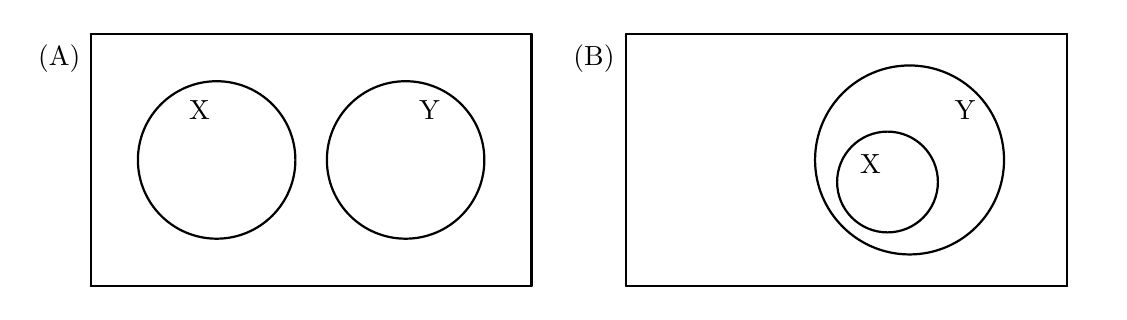
\begin{tikzpicture}[line width=0.8pt,line cap=round,line join=round,>=triangle 45,x=1.0cm,y=1.0cm,scale=0.4]
%\clip(-7,-4.2) rectangle (10,4.2);
\clip(-7,-4.2) rectangle (27,4.2);
\draw (-1.,0.) circle (2.5cm);
\draw (5,0.) circle (2.5cm);
\draw (-5.,4.)-- (-5.,-4.);
\draw (-5.,-4.)-- (9.,-4.);
\draw (9.,-4.)-- (9.,4.);
\draw (9.,4.)-- (-5.,4.);
\draw (-2.2,2.2) node[anchor=north west] {X};
\draw (5.1,2.2) node[anchor=north west] {Y};
\draw (-7,4) node[anchor=north west] {(A)};

\begin{scope}[shift={(17,0)}]
\draw (3.3,-0.7) circle (1.6cm);
\draw (4.,0.) circle (3.cm);
\draw (-5.,4.)-- (-5.,-4.);
\draw (-5.,-4.)-- (9.,-4.);
\draw (9.,-4.)-- (9.,4.);
\draw (9.,4.)-- (-5.,4.);
\draw (2.1,0.5) node[anchor=north west] {X};
\draw (5.1,2.2) node[anchor=north west] {Y};
\draw (-7,4) node[anchor=north west] {(B)};
\end{scope}

\end{tikzpicture}

%\begin{image}
%  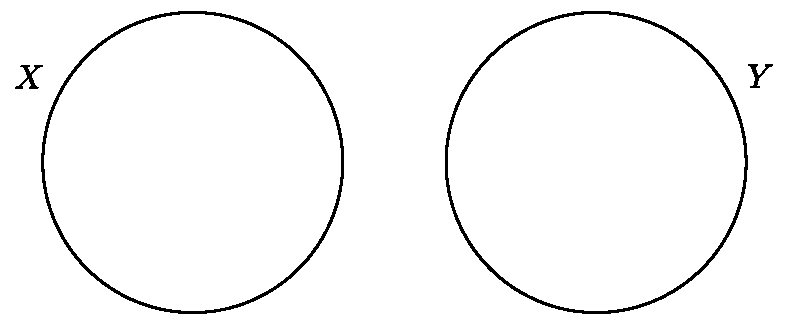
\includegraphics{set4.png}
%\end{image}
\begin{enumerate}
\item If Venn diagram (A) above shows the relationship between sets $X$ and $Y$, then $X\cap Y =$ \wordChoice{\choice{$0$}\choice[correct]{$\emptyset$}\choice{$X\cup Y$}} and the sets are said to be 
\wordChoice{\choice[correct]{disjoint}\choice{empty}\choice{subsets}}.  

\item If Venn diagram (B) above shows the relationship between sets $X$ and $Y$, then we say that \wordChoice{\choice{$X$ and $Y$ are disjoint}\choice[correct]{$X\subseteq Y$}\choice{$Y\subseteq X$}}.

\item If we let $X$ be the set of ``right triangles'' and we let $Y$ be the set of ``equilateral triangles'' which diagram above shows the relationship between these two sets?
\begin{multipleChoice}
\choice[correct]{Diagram (A).}
\choice{Diagram (B).}
\choice{Neither of these.}
\choice{Not enough information.}
\end{multipleChoice}

Explain your reasoning.
\begin{freeResponse}
\begin{hint}
Diagram (A) is accurate because no right triangles are also equilateral triangles.  
\end{hint}
\end{freeResponse}
\end{enumerate}
\end{problem}


\begin{problem}
If $X = \{1,2,3,4,5\}$ and $Y = \{3,4,5,6\}$ find the following: (List elements in ascending order, separated by commas, with no spaces.)
\begin{enumerate}
\item $X\cup Y = \{\answer[format=string]{1,2,3,4,5,6}\}$
\item $X\cap Y = \{\answer[format=string]{3,4,5}\}$
\item $X-Y = \{\answer[format=string]{1,2}\}$
\item $Y-X = \{\answer[format=string]{6}\}$
\end{enumerate}
\end{problem}

\begin{problem}
Let $n\mathbb Z$ represent the integer multiples of $n$. So for example:
\[
3\mathbb Z = \{\dots,-12,-9,-6,-3,0,3,6,9,12,\dots\}
\]
Compute the following (use capital $Z$ for $\mathbb Z$):
\begin{enumerate}
\item $3\mathbb Z\cap 4\mathbb Z = \answer{12Z}$ 
\item $2\mathbb Z\cap 5\mathbb Z = \answer{10Z}$
\item $3\mathbb Z\cap 6\mathbb Z = \answer{6Z}$
\item $4\mathbb Z\cap 6\mathbb Z = \answer{12Z}$
\item $4\mathbb Z\cap 10\mathbb Z = \answer{20Z}$
\end{enumerate}
\end{problem}

%\begin{problem}
%Let $n\Z$ represent the integer multiples of $n$. So for example:
%\[
%3\Z = \{\dots,-12,-9,-6,-3,0,3,6,9,12,\dots\}
%\]
%Compute the following (use capital $Z$ for $\Z$):
%\begin{enumerate}
%\item $3\Z\cap 4\Z = \answer{12Z}$ 
%\item $2\Z\cap 5\Z = \answer{10Z}$
%\item $3\Z\cap 6\Z = \answer{6Z}$
%\item $4\Z\cap 6\Z = \answer{12Z}$
%\item $4\Z\cap 10\Z = \answer{20Z}$
%\end{enumerate}
%\end{problem}

\begin{problem}
Make a general rule for intersecting sets of the form $n\mathbb Z$ and
  $m\mathbb Z$. Explain why your rule works.
\begin{freeResponse}
\begin{hint}
The intersection of two sets is what they have in \emph{common}.  The intersection of the set of multiples of $n$ and the set of multiples of $m$ are called \emph{common multiples} (surprise!), and they are all multiples of the least common multiple of $n$ and $m$.  
\end{hint}
\end{freeResponse}
\end{problem}

\begin{problem}
If $X\cup Y = X$, what can we say about the relationship between the sets $X$ and $Y$? Explain your reasoning.

% $Y\subseteq X$ because every element of $Y$ must already be in $X$.  
\wordChoice{\choice{$X\subseteq Y$}\choice{$X=Y$}\choice[correct]{$Y\subseteq X$}\choice{$X=\emptyset$}}
because every element of \wordChoice{\choice{$X$}\choice[correct]{$Y$}} must be in \wordChoice{\choice[correct]{$X$}\choice{$Y$}}.

\end{problem}

\begin{problem}
If $X\cap Y = X$, what can we say about the relationship between the sets $X$ and $Y$? Explain your reasoning.

% $X\subseteq Y$ because every element of $X$ must already be in $Y$. 
\wordChoice{\choice[correct]{$X\subseteq Y$}\choice{$X=Y$}\choice{$Y\subseteq X$}\choice{$X=\emptyset$}}
because every element of \wordChoice{\choice[correct]{$X$}\choice{$Y$}} must be in \wordChoice{\choice{$X$}\choice[correct]{$Y$}}.
\end{problem}

\begin{problem}
If $X-Y =\emptyset$, what can we say about the relationship between the sets $X$ and $Y$? Explain your reasoning.

% $X\subseteq Y$ because that would mean $X$ contains no elements that are not also in $Y$.
\wordChoice{\choice[correct]{$X\subseteq Y$}\choice{$X=Y$}\choice{$Y\subseteq X$}\choice{$X=\emptyset$}}
because every element of \wordChoice{\choice[correct]{$X$}\choice{$Y$}} must be in \wordChoice{\choice{$X$}\choice[correct]{$Y$}}.
\end{problem}



\end{document}
